\documentclass[11pt]{article}
\usepackage[top=1in, bottom=1in, left=1in, right=1in]{geometry}
\usepackage{amsmath}
\usepackage{amssymb}
\usepackage{graphicx}
\usepackage{titlesec}
\titleformat{\subsection}[runin]{\normalfont\large\bfseries}{\thesubsection}{1em}{}

\begin{document}
\pagestyle{empty}
%\parindent=0pt

\section*{\centering Problem Set 11 (part 1)}

\section{Dust Temperatures and Opacity}

The bulk of the interstellar radiation field in the Galaxy is from the light of
O stars, which have mass $\sim100M_\odot$.  There are $\sim5\times10^4$ O stars in the galaxy,
distributed over a cylindrical disk with radius 50 kpc and height 200 pc.

\subsection{}
Estimate the total energy density of starlight in the Galaxy in units of eV~cm$^{-3}$.
Use the fact that O stars radiate near the Eddington luminosity.

\subsection{}
This interstellar radiation field heats dust grains in the interstellar medium.
Estimate the temperature $t$ of the largest grains in the ISM, which have a radius
of $a\sim0.1$ microns.  Assume $Q_{abs}\sim1$ for wavelengths shorter than $2\pi a$,
and for longer wavelengths, take $m=1+0.25i$.
Is the grain hotter, cooler, or equal
to the temperature of an ideal blackbody placed in the interstellar radiation field.

\subsection{}
At what wavelength, $\lambda_{peak}$, does the energy density $(\nu F_\nu)$ of the grains peak?

\subsection{}
The largest grains carry most of the mass in the interstellar grain distribution.
Given a dust-to-gas ratio of $0.01$ and an average hydrogen number density
$n_H=0.1 {\rm cm}^{-1}$, calculate the specific intensity of the Milky Way
at $\lambda_{peak}$.

\subsection{}
Typically, the number density of dust grains scales with size as $dn/da\propto a^{-3.5}$ in
the ISM, where $dn$ is the number density of grains with radii between $a$ and $a+da$.  The
law holds over $a_{min}=10^{-3}$ microns to $a_{max}=0.1$ microns.  Plot the grain opacity
$\kappa(\lambda)$ contributed by all dust grains over the wavelength range $\lambda=0.1$ to
10 microns.  Consider only absorption and neglect scattering.  Indicate over each decade of
wavelength which grain sizes dominate the opacity.


\section*{Problem Set 10 (part 2)}

\section{Diatomic}

Based on Rybicki \& Lightman 11.1.

Consider an electrically neutral medium of diatomic molecules in thermal equilibrium at
temperature $T$.  Each molecule contains one nucleus of mass $m_p$ and one of mass $2m_p$
at an equilibrium separation $r_0$.

\subsection{}
Estimate $r_0$ in terms of fundamental constants.

\subsection{}
Estimate the cross-section $\sigma_c$ for collisions between molecules.

\subsection{}
\begin{figure}
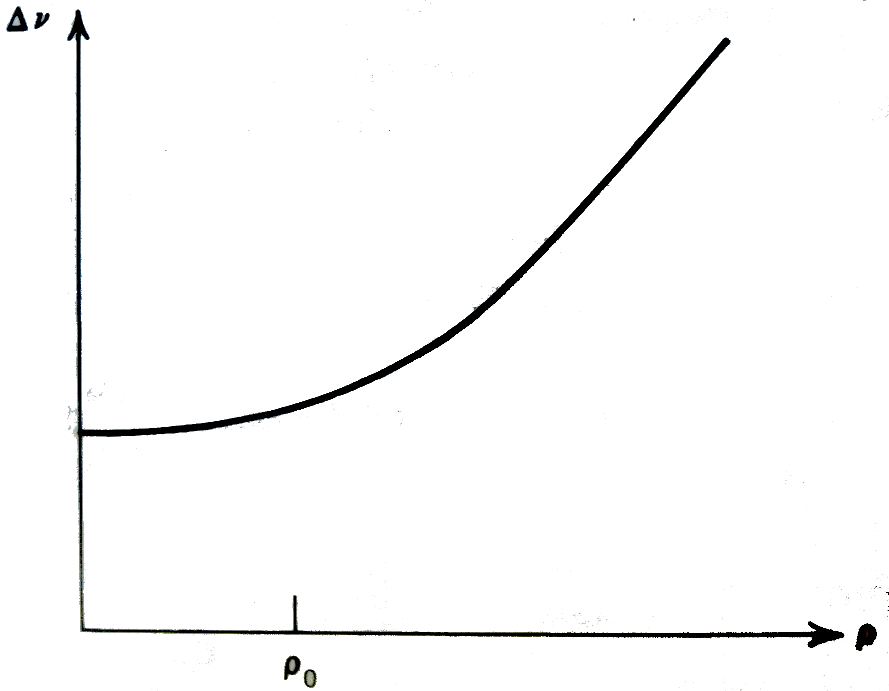
\includegraphics[width=3in]{ps11_linewidth.png}
\caption{
Line width as a function of denisty for emission from a medium of diatomic molecules.
}\label{fig:linewidth}
\end{figure}

It is experimentally observed that , as a function of mass density $\rho$ of
the medium, the line width of the rotational lines has the form
shown in Figure \ref{fig:linewidth}.  If only Doppler and collisional broadening
are present, estimate $\rho_0$ and show that it may be written completely in
terms of fundamental constants, independent of $m_p$. 

We derived in class that for a synchrotron self-Compton (SSC) emitting source
that is static in bulk, the ratio of the luminosity due to first-generation
inverse Compton scattering of synchrotron photons to the luminosity due to synchrotron processes is
\begin{equation}
f\equiv\frac{L_{IC,1}}{L_{sync}}=C\nu_mT_{bm}^5
\end{equation}
where $\nu_m$ is the frequency at which the synchrotron spectrum beaks, and $T_{bm}$
is the brightness temperature of the synchrotron radiation at that frequency.

\subsection{}
Derive an estimate for the constant $C$ in terms of fundamental constants.
Assume whatever geometry you like for the source.  I found I had to use the (usual)
constants $e$, $k$, $c$, and $m_e$.

\subsection{}
If $\nu_m\sim1~{\rm GHz}$ (as it typically is for compact radio sources), what is the
maximum $T_{bm}$ above which $f>1$?  Express in Kelvin.

\subsection{}
Given $f$, what is $L_{IC,2}/L_{IC,1}$?  That is, what is the ratio of second-generation
to first-generation scattered power?  Explain your answer.

\subsection{}
Consider the situation after $N$ scatterings, where $N\rightarrow\infty$.  What is the 
critical $f$ for which the total luminosity of the source becomes unbounded?  Careful
estimates will be rewarded.

\end{document}
